\subsubsection{Évolutions simples}
\label{exo_evolutions_simples}

	(un exercice simplement destiné à mettre en pratique les conventions de signe et le vocabulaire du cours)

	Une masse de~\SI{400}{\gram} d’eau est placée dans un réservoir hermétique. Elle suit une évolution pendant laquelle elle reçoit \SI{50}{\kilo\joule\per\kilogram} de chaleur et voit son énergie interne augmenter de~\SI{4}{\kilo\joule}.
	
	\begin{enumerate}
		\item A-t-elle reçu ou fourni du travail, et en quelle quantité ?
	\end{enumerate}
	
	On fournit ensuite à cette même masse un travail de~\SI{800}{\joule} de manière adiabatique.
	
	\begin{enumerate}
		\shift{1}
		\item Quelle est la variation de son énergie interne spécifique ?
	\end{enumerate}
	

\subsubsection{Évolutions arbitraires d’un gaz en laboratoire}
\label{exo_evolutions_arbitraires}

	Une masse de~\SI{80}{\gram} d’hélium est contenue dans un cylindre de~\SI{0,04}{\metre\cubed}. Le gaz est d’abord refroidi de façon réversible à pression constante jusqu’à~\SI{0,02}{\metre\cubed} et~\SI{2}{\bar} ; puis réchauffé à volume constant jusqu’à~\SI{4}{\bar}.
	
	\begin{enumerate}
		\item Tracez l’évolution sur un diagramme pression-volume.
		\item Quel est le travail fourni ou reçu par le gaz ?
	\end{enumerate}


\subsubsection{Suspension pneumatique de camion}
\label{exo_pneumatique_camion}

	Le système de suspension pneumatique d’une remorque de camion peut être modélisée avec un cylindre d’air. Lorsque la remorque est chargée, le piston fixé à la remorque descend à l’intérieur du cylindre qui est fixé à l’arbre des roues, écrasant l’air qui y est prisonnier (\cref{fig_camion}).

	\begin{figure}
	\begin{center}
		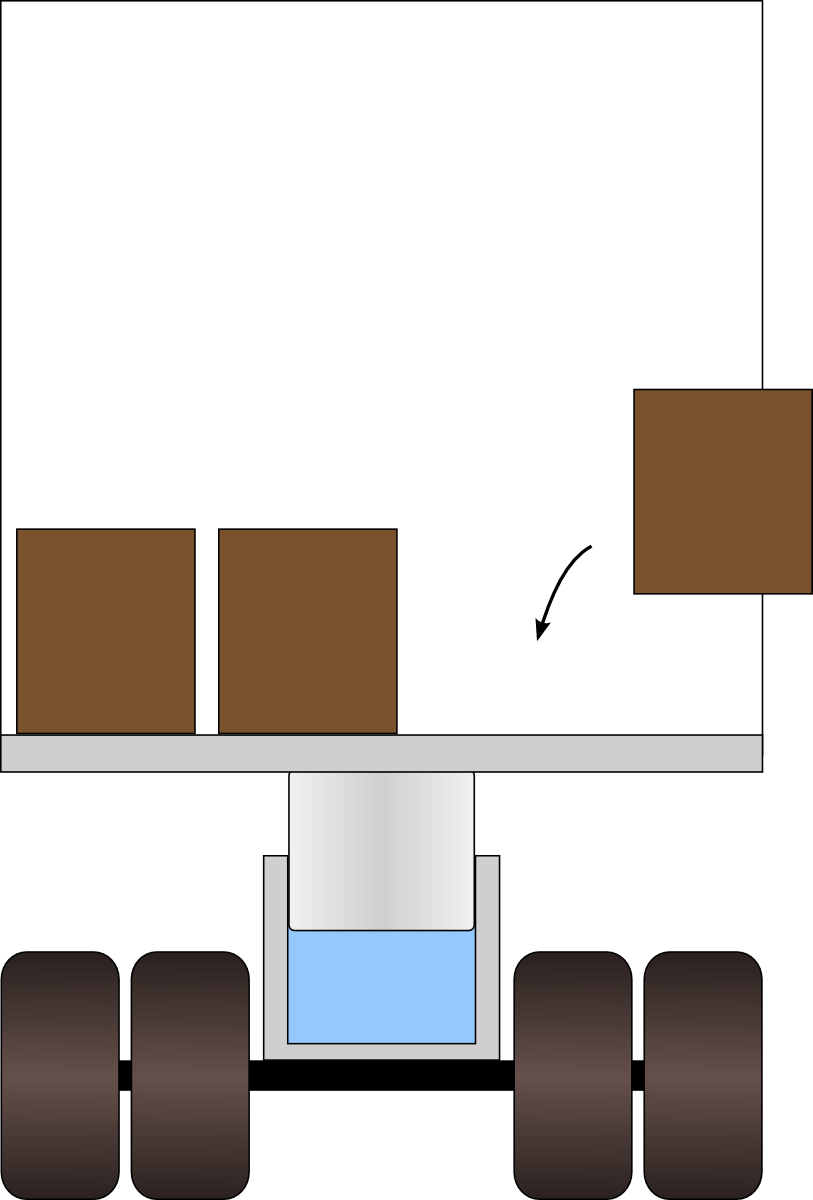
\includegraphics[height=8cm]{images/piston_camion.png}
	\end{center}
		\supercaption{Modélisation schématique d’un système de suspension pneumatique de camion. Le piston, au centre, comprime une masse d’air (en bleu) lorsque la remorque est chargée.}{schéma \cczero \oc}
	\label{fig_camion}
	\end{figure}
	
	Dans un premier temps on charge le camion très progressivement. L’air à l’intérieur du cylindre ne perd ni reçoit de chaleur. Ses caractéristiques évoluent alors selon la relation $p v^{1,4} = \num{5,438e4}$ (en unités \textsc{si}).
	
	La compression commence à $p_\A = \SI{2,5}{\bar}$. Lorsque le chargement est terminé, la pression est montée à $p_\B = \SI{10}{\bar}$.
	
	\begin{enumerate}
		\item Représentez l’évolution du gaz pendant le chargement sur un diagramme pression-volume, de façon qualitative (c’est-à-dire sans représenter les valeurs numériques).
		\item Le travail effectué par une force $\vec F$ sur un déplacement $\vec l$ s’exprime selon
			\begin{equation}
				W \equiv \vec F \cdot \vec l 	\tag{\ref{eq_travail_fdl}}
			\end{equation}
			À partir de cette équation, exprimez le travail effectué sur un corps de masse fixe en fonction de son volume spécifique et de sa pression interne.
		\item Combien d’énergie le gaz a-t-il reçu pendant le chargement ?
		\item Quelle énergie le gaz fournirait-il en retour si le camion était déchargé très progressivement ?
	\end{enumerate}
	
	On décharge brutalement le camion et le piston remonte rapidement jusqu’à ce que la pression finale redescende à sa valeur initiale.
	
	\begin{enumerate}
		\setcounter{enumi}{3}
		\item Représentez l’évolution sur le diagramme pression-volume précédent, de façon qualitative.
		\item Que peut-on faire pour ramener le gaz à l’état exact où il était avant le chargement ?
	\end{enumerate}


\subsubsection{Compresseur à air}
\label{exo_compresseur_air}

	Dans un petit compresseur à air (\cref{fig_compresseur}), un piston comprime lentement et sans frottement une masse fixe d’air. Le cylindre est muni d’aubes, qui permettent de dissiper de la chaleur. Ainsi, la compression se fait à énergie interne constante.	

	\begin{figure}[h]%FIXME: cette figure doit être *dans* l’exo plutôt que au dessus
	\begin{center}
		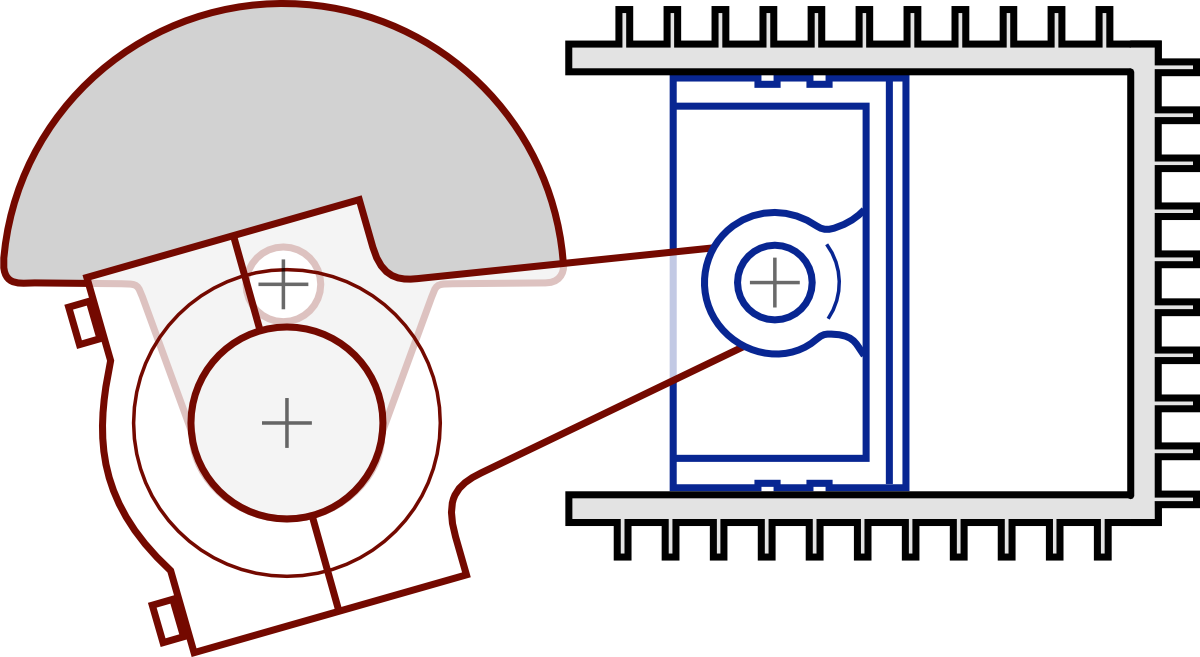
\includegraphics[width=8cm]{images/compresseur_air.png}
	\end{center}
	\supercaption{Schéma de coupe d’un petit compresseur à air à piston. Les soupapes d’admission et de sortie ne sont pas représentées.}{Schéma \ccbysa \wcfile{Piston_bielle_vilebrequin_coupe_et_schema_cinematique.svg}{Christophe Dang Ngoc Chan} \& \olivier}
	\label{fig_compresseur}
	\end{figure}

	On dépense, pour la compression de l’air, un travail de~\SI{150}{\kilo\joule\per\kilogram}.
		
	\begin{enumerate}
		\item Quel est le transfert de chaleur pendant la compression ?
	\end{enumerate}
	
	Avant de commencer la compression, l’air est à pression et masse volumique atmosphériques (\SI{1}{\bar} ; \SI{1,2}{\kilogram\per\metre\cubed}). Le diamètre du cylindre est de~\SI{5}{\centi\metre} et sa profondeur intérieure est de~\SI{15}{\centi\metre}.
	
	\begin{enumerate}
		\shift{1}
		\item Quelle est la masse d’air incluse dans le cylindre ?
	\end{enumerate}


	Pendant la compression, on observe que la pression et le volume spécifique sont liés par la relation $p v = k$ (où $k$ est une constante).

	\begin{enumerate}
		\shift{2}
		\item À quelle pression va-t-on pouvoir mener l’air à la fin de la compression ?
	\end{enumerate}


\subsubsection{Cycle d’un moteur à essence}
\label{exo_cycle_moteur_essence}

	On souhaite étudier le fonctionnement d’un moteur à essence à quatre cylindres (\cref{fig_exo_pistons}). Comme tous les moteurs thermiques alternatifs, il dégage du travail en faisant varier la pression et le volume de petites quantités d’air emprisonnées dans ses cylindres. Nous simplifions ici les détails de son fonctionnement pour le réduire au cas idéal, dans lequel les évolutions sont toutes réversibles.
	
	Le moteur a pour cylindrée \SI{1,1}{\liter} ; il est muni de quatre cylindres de diamètre \SI{7}{\centi\metre} et a un taux de compression (rapport entre volumes maximum et minimum dans un cylindre) de~\num{7,9}. L’air pénètre dans le moteur aux conditions atmosphériques (\SI{1}{\bar}, \SI{0,84}{\metre\cubed\per\kilogram}).
	
		\begin{figure}
			\begin{center}
				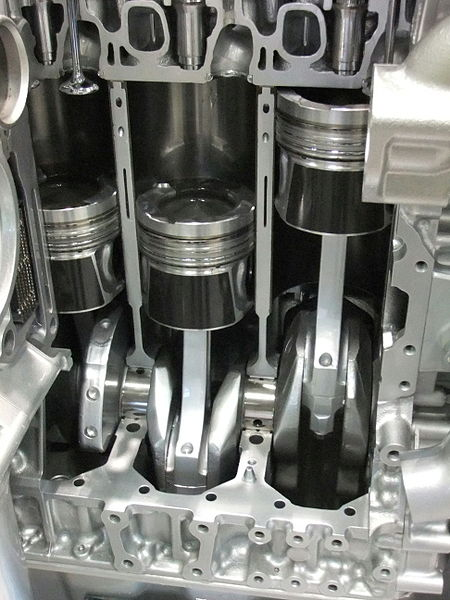
\includegraphics[width=6cm, max width=0.8\columnwidth]{images/pistons_cutaway.jpg}
			\end{center}
			\supercaption{Pistons et cylindres d’un moteur automobile découpé.}{\wcfile{Internal combustion engine pistons of partial cross-sectional view.jpg}{Photo} \ccbysa par \wcu{Mj-bird}}
			\label{fig_exo_pistons}
		\end{figure}
	
	Nous pouvons décrire un cycle à l’intérieur d’un cylindre avec les quatre étapes suivantes :
	
	\begin{description}
			\item [De A à B] l’air est comprimé de façon adiabatique réversible depuis le point mort bas jusqu’au point mort haut. Pendant cette évolution, nous savons que ses propriétés sont liées par la relation $p \ v^{k_1} = k_2$. En B, la pression a atteint \SI{16,97}{\bar}.
			\item [De B à C] il est chauffé à volume constant (comme si le piston était immobilisé), jusqu’à ce que la pression atteigne~\SI{75}{\bar}. En mesurant la température on constate que son énergie interne spécifique augmente de~\SI{1453,3}{\kilo\joule\per\kilogram}.
			\item [De C à D] l’air est détendu de façon adiabatique réversible depuis le point mort haut jusqu’au point mort bas. Ses propriétés sont liés par la relation $p \ v^{k_1} = k_3$.
			\item [De D à A] il est refroidi à volume constant (comme si le piston était immobilisé), jusqu’à retrouver ses propriétés en A.\\
				(En pratique, cette phase de refroidissement a lieu hors du moteur, dans l’atmosphère. Elle peut toutefois être modélisée ainsi sans induire d’erreur.)
	\end{description}

	\begin{enumerate}
		\item Représentez le cycle suivi par l’air sur un diagramme pression-volume, de façon qualitative.
		\item {Quelle est la masse d’air présente dans un cylindre ?\\
				{\tiny indice : $V_\text{cylindrée} = 4 (V_\text{cylindre max.} - V_\text{cylindre min.}) = 4 (V_\text{point mort bas} - V_\text{point mort haut})$}}
		\item Quel est le travail spécifique reçu par l’air pendant la compression (de A à B) ?
		\item Quelle est la chaleur spécifique reçue par l’air pendant la combustion (de B à C) ?
		\item Quel est le travail spécifique dégagé par l’air pendant la détente (de C à D) ?
		\item Quelle est la chaleur spécifique rejetée par l’air pendant la phase de refroidissement ?
		\item Quelle est l’efficacité du moteur, c’est à dire le rapport entre le travail net dégagé pendant le cycle et la chaleur fournie pendant la combustion ?
		\item Combien faut-il effectuer de cycles par seconde pour que le moteur dégage une puissance de~\SI{80}{\cheval} (\SI{58,84}{\kilo\watt}) ?
	\end{enumerate}



\subsubsection{Travail dans un moteur diesel}
\label{exo_quatre_cylindres}
	
	Nous étudions le fonctionnement d’un moteur alternatif à quatre cylindres en modélisant son fonctionnement dans le cas le plus favorable, c’est à dire avec des évolutions très lentes (parfaitement réversibles).

	\begin{figure}
		\begin{center}
			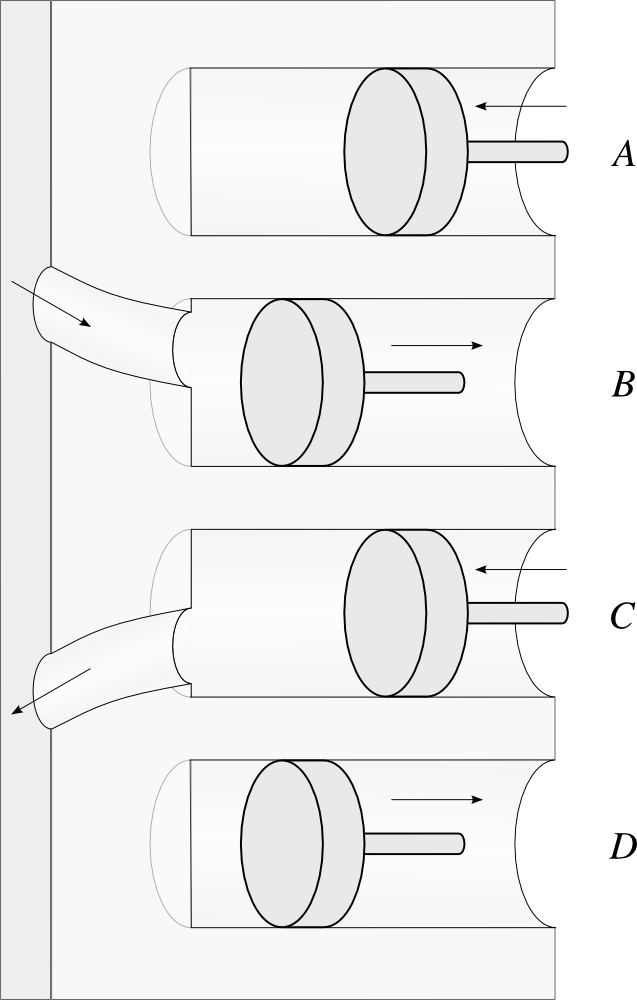
\includegraphics[width=8cm]{images/quatre_cylindres.png}
		\end{center}
		\supercaption{Représentation schématique du fonctionnement d’un moteur à quatre cylindres. Les pistons A et C sont en remontée, et les pistons B et D sont en descente. Ils sont tous les quatre liés au même axe moteur, non représenté ici.}{Schéma \ccbysa \olivier}
		\label{fig_quatre_cylindres}
	\end{figure}
	
	À l’intérieur du bloc moteur schématisé en \cref{fig_quatre_cylindres}, quatre pistons liés à l’axe moteur par un vilebrequin (non représenté) sont en mouvement. L’évolution est différente dans chaque cylindre :
	
	\begin{description}
		\item [Cylindre A :] {compression (l’air restant prisonnier du cylindre).\nopagebreak\\
									La compression de l’air débute à~\SI{0,8}{\bar} et ses y sont liées par la relation $p V^{\num{1,3}} = k_1$.}
		\item [Cylindre B :] {admission.\\
									L’air est admis à pression constante de~\SI{0,8}{\bar}.}
		\item [Cylindre C :] {échappement.\\
									L’air est rejeté à pression constante de~\SI{1,1}{\bar}.}
		\item [Cylindre D :] {détente.\\
									L’air à haute pression et température est prisonnier du cylindre ; ses propriétés sont aussi reliées par la relation $p V^{\num{1,3}} = k_2$.}
	\end{description}
		
		Bien sûr, le rôle de chaque cylindre change deux fois par tour. Nous étudions ici les transferts de travail sur un demi-tour moteur.

		Même si les cylindres B et C ne sont pas des systèmes fermés, pour les besoins de l’exercice nous pouvons modéliser leurs évolutions comme si c’était le cas, sans induire d’erreur.

		Les conditions atmosphériques sont de~\SI{1}{\bar} et~\SI{1,225}{\kilogram\per\metre\cubed}.	La cylindrée du moteur est de~\SI{1,5}{\liter} et le taux de compression (c’est à dire le rapport des volumes minimal et maximal au sein de chaque cylindre) est de~\num{22}.
		
		\begin{enumerate}
			\item Représentez l’évolution dans chacun des cylindres sur un même diagramme pression-volume, de façon qualitative.
			\item Quelle est l’énergie nécessaire pour déplacer les cylindres B et C ?
			\item Quelle est l’énergie reçue par le gaz dans le cylindre A ?
		\end{enumerate}
		
		On souhaite que le moteur développe une puissance de~\SI{30}{\kilo\watt} à vitesse de~\num{2000} \si{tours/min}. Ses pertes mécaniques sont de l’ordre de~\SI{15}{\percent}.
		
		\begin{enumerate}
			\shift{3}
			\item Quel est le travail qui doit être développé par le cylindre D pendant la détente ?
			\item À quelle pression la combustion de l’essence dans le cylindre D doit-elle y porter l’air, pour que la détente puisse faire fonctionner le moteur ?
		\end{enumerate}



\subsubsection{Prendre de la chaleur où il fait plus froid}
\label{exo_prendre_de_la_chaleur}

	Un/e étudiant/e tente une expérience avec un peu d’air dans un cylindre, dont il/elle contrôle le volume avec un piston. Le but est de prélever de la chaleur à l’extérieur, où la température est basse, pour la rejeter à l’intérieur de la pièce.

	La masse d’air emprisonnée dans le cylindre est de~\SI{6e-3}{\kilogram}.
	
	Au départ, l’air dans le cylindre occupe un volume de~\SI{0,5}{\liter}. La pression et la température sont celles de la pièce (\SI{1}{bar} ; \SI{18}{\degreeCelsius}).

	\begin{description}
		\item[de A à B] L’étudiant/e isole bien le cylindre avec un isolant thermique, et détend lentement le gaz en augmentant son volume jusqu’à~\SI{4,5}{\liter}. Nous savons\footnote{Nous verrons d’où vient cette relation et apprendrons à calculer cette température au \coursquatre.} que, pendant ce type de détente, la pression et le volume sont liés par la relation
			\begin{equation*}
				p v^{1,4} = k_2
			\end{equation*}
			 où $k_2$ est une constante.
		
			La température du gaz chute dramatiquement pendant la détente\ – en B le thermomètre indique finalement $T_\B = \SI{121}{\kelvin}$.
		
		\item[de B à C]	L’étudiant/e fixe le volume du cylindre en bloquant mécaniquement le piston, retire l’isolant thermique, et pose le cylindre au dehors du bâtiment (température extérieure : \SI{-5}{\degreeCelsius}). La température et la pression du gaz remontent doucement.

		\item[de C à A] Lorsque la pression atteint \SI{1}{\bar} précisément, la température de l’air est indiquée à~$T_\C = \SI{262}{\kelvin}$. 	
					
			L’étudiant/e souhaite revenir aux conditions de départ (en réduisant le volume jusqu’au volume initial) en gardant la pression constante à~\SI{1}{\bar}.
	\end{description}.
	
	\begin{enumerate}
		\item Schématisez l’évolution sur un diagramme pression-volume.
		\item {Montrez que lors d’une évolution réversible d’un sytème fermé dont les propriétés sont liées par une relation de type $p v^{k_1} = k_2$ (où $k_1 \neq 1$ et $k_2$ sont des constantes), le travail spécifique développé est :
				\begin{equation*}
				w_{\A\to\B} = \frac{p_\B v_\B - p_\A v_\A}{k_1 - 1}
				\end{equation*}}
		\item Quel est le travail spécifique fourni par le gaz pendant la détente ?
		\item La capacité thermique de l’air lorsque l’on bloque son volume est égale à~\SI{718}{\joule\per\kilo\gram\per\kelvin}. Quelle quantité de chaleur a-t-elle été rejetée ou prélevée de l’air extérieur ?
		\item Quelle quantité de travail sera nécessaire pour effectuer le retour C$\to$ A à pression constante ?
		\item Sur l’entièreté du cycle, l’étudiant/e aura-t-il/elle dépensé ou reçu du travail ?
		\item {[question difficile]} Le chemin du retour à pression constante nécessite un transfert de chaleur. Dans quel sens, et en quelle quantité ? Pourquoi ce transfert ne peut-t-il (malheureusement) pas être entièrement effectué à l’intérieur du bâtiment ?
	\end{enumerate}



\exercisesolutionpage
\titreresultats

\begin{description}
	\item [\ref{exo_evolutions_simples}]
					\tab 1) $W_\fromatob = \Delta U - m q_\fromatob = \SI{-16}{\kilo\joule}$ (donc un travail fourni)
					\tab 2) $\Delta u = q_\frombtoc + w_\frombtoc =  0 + \frac{W_\frombtoc}{m} = \SI{+2}{\kilo\joule\per\kilogram}$.
	\item [\ref{exo_evolutions_arbitraires}]
					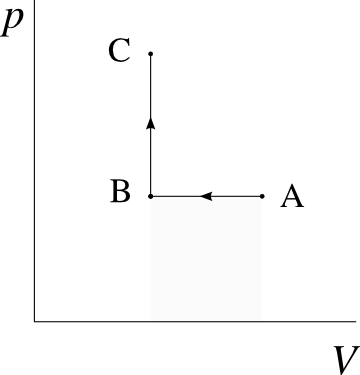
\includegraphics[width=\solutiondiagramwidth]{images/exo_sol_pv_1.png}
					\tab 2) $W_{\A\to\C} = W_\fromatob + W_\frombtoc = -p_{\text{cste.}} \left[V\right]_{V_\A}^{V_\B } + 0 = \SI{+4}{\kilo\joule}$
	\item [\ref{exo_pneumatique_camion}]
					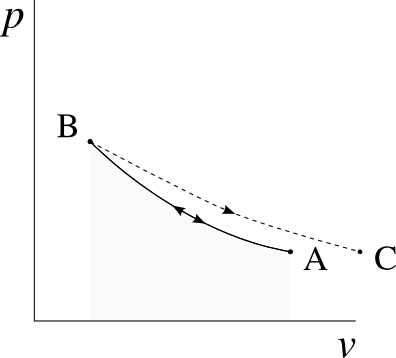
\includegraphics[width=\solutiondiagramwidth]{images/exo_sol_pv_camion.png}
					\tab 2) voir \S\ref{ch_travail_pdv} \& \S\ref{ch_travail_fdl}
					\tab 3) $v_\A = \SI{0,336}{\metre\cubed\per\kilogram}$ et $v_\B = \SI{0,125}{\metre\cubed\per\kilogram}$ ; ainsi $w_\fromatob = -k \left[\frac{1}{\num{-0,4}} v^{\num{-0,4}}\right]_{v_\A}^{v_\B } = \SI{+102,1}{\kilo\joule\per\kilogram}$.
					\tab 4) $w_\frombtoa =  - w_\fromatob$
					\tab 5) Un refroidissement à pression constante, par exemple.
	\item [\ref{exo_compresseur_air}]
					\tab 1) $q_\fromatob = \Delta u - w_\fromatob = - w_\fromatob$.
					\tab 2) $m = \frac{V_\A}{v_\A} = \SI{3,534e-4}{\kilogram}$
					\tab 3) $\frac{v_\B }{v_\A} = \exp \left[-\frac{w_\fromatob}{k}\right]$ ; ainsi $p_\B = p_\A \frac{v_\A}{v_\B } = \SI{6,05}{\bar}$
	\item [\ref{exo_cycle_moteur_essence}]
					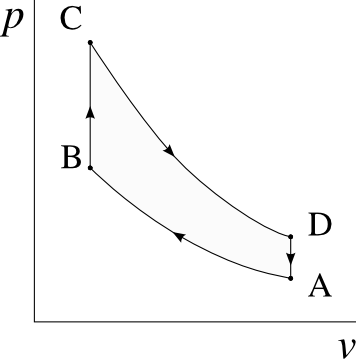
\includegraphics[width=\solutiondiagramwidth]{images/exo_sol_pv_moteur_essence.png}
					\tab 2) $V_\A = \SI{3,149e-4}{\metre\cubed}$ ; ainsi $m_\A = \frac{V_\A}{v_\A} = \SI{3,748e-4}{\kilogram}$
					\tab 3) $k_1 = \num{1,3699}$ et $k_2 = \SI{7,8753e4}{\usi}$ ; ainsi $w_\fromatob = -k_2 \left[\frac{1}{-k_1 + 1} v^{-k_1 + 1} \right]_{v_\A}^{v_\B } = \SI{+260,7}{\kilo\joule\per\kilogram}$.
					\tab 4) $q_\frombtoc = \Delta u - w_\frombtoc = \Delta u - 0 = \SI{+1543,3}{\kilo\joule\per\kilogram}$
					\tab 5) $w_\fromctod = -k_3 \left[\frac{1}{-k_1 + 1} v^{-k_1 + 1} \right]_{v_\C}^{v_\D} = -\frac{k_3}{k_2} w_\fromatob = -\frac{p_\C}{p_\B } w_\fromatob = \SI{-1152,2}{\kilo\joule\per\kilogram}$
					\tab 6) $q_\fromdtoa = -w_\fromatob - q_\frombtoc - w_\fromctod = \SI{-651,8}{\kilo\joule\per\kilogram}$
					\tab 7) $\eta_{\text{moteur}} = \left|\frac{w_\fromatob + w_\fromctod}{q_\frombtoc}\right| = \SI{57,8}{\percent}$ (très honorable)
					\tab 8) $f = \frac{\dot W_{\text{moteur}}}{m_\A \ (w_\fromatob + w_\fromctod)} = \SI{176,1}{\hertz}$ (176 combustions par seconde), soit environ \SI{5300}{tours par minute} avec un moteur quatre cylindres à quatre temps.
	\item [\ref{exo_quatre_cylindres}]
					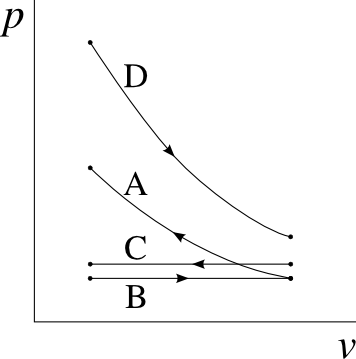
\includegraphics[width=\solutiondiagramwidth]{images/exo_sol_pv_quatre_cylindres.png}
					\tab 2) $W_{\text{cyl. B}} = -p_\B \left[V\right]_{V_\text{min.}}^{V_\text{max.}} = - p_\B \left(\frac{V_\text{cylindrée}}{4}\right) = \SI{-30}{\joule}$ ; $W_{\text{cyl. B}} =  \SI{-41,3}{\joule}$
					\tab 3) $V_\text{A1} = \frac{22}{21\times4}V_\text{cylindrée} = \SI{3,9286e-4}{\metre\cubed}$ et $V_\text{A2} = \frac{V_\text{A1}}{22} = \SI{1,7857e-5}{\metre\cubed}$. Ainsi, $k_1 = \SI{2,9895}{\usi}$, et enfin $W_{\text{cyl. A}} = \frac{k_1}{\num{0,3}} \left(V_\text{A2}^{\num{-0,3}} - V_\text{A1}^{\num{-0,3}}\right) = \SI{+185,5}{\joule}$.
					\tab 4) $\dot n = \SI{2000}{rpm} = \SI{33,3}{rps}$ : il y a donc \num{66,7} évolutions par seconde ($f = \SI{66,7}{\hertz}$). On obtient $W_\text{4 cylindres} = \frac{1}{f} \frac{1}{\eta_\text{méca.}} \dot W_\text{moteur}$ ; et enfin $W_\text{cyl. D} = W_\text{4 cylindres} - W_\text{cyl. A} - W_\text{cyl. B} -W_\text{cyl. C} = \SI{-726,2}{\joule}$.
					\tab 5) On calcule $k_2$ à partir de $W_\text{cyl. D}$, et on obtient $p_\text{D1} = \SI{173,9}{\bar}$.
	\item [\ref{exo_prendre_de_la_chaleur}]
					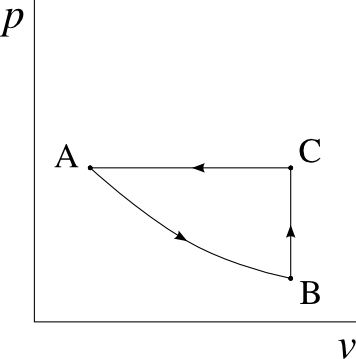
\includegraphics[width=\solutiondiagramwidth]{images/exo_sol_pv_prelever.png}
					\tab 3) Ayant obtenu $p_\B = \SI{4,61e-2}{\bar}$, on calcule $W_\fromatob = \frac{p_\B V_\B - p_\A V_\A}{k_1 - 1} = \SI{-73,14}{\joule}$.
					\tab 4) $Q_\frombtoc = m c_v \Delta T = \SI{+607,4}{\joule}$
					\tab 5) $W_{\C \to \A} = \SI{+400}{\joule}$ (facile!)
					\tab 5) $W_\text{cycle} = \SI{+326,86}{\joule}$, donc une dépense de l’étudiant/e.
					\tab 6) $Q_{\C \to \A} = \SI{-934,26}{\joule}$
					\tab 7) C’est une histoire de température\ldots
\end{description}

